\section{Intepretation}
\label{sec:Interpretation}

In general, the bright and hard gamma-ray emission at the base of the bubbles can be at any position along the line of sight.
In this section we consider two characteristic scenarios: that the emission is near the GC or that the emission is 
produced by one or a few SNRs closer to us. 
% (similar to, e.g., the Cygnus region that contains recently accelerated CRs from several SNRs).

\subsection{Emission near the GC scenario}
\lb{sec:GC_scenario}

In the estimates in this subsection we use the following characteristic sizes: 
the distance to the GC is $\SI{8.5}{kpc}$, 
the size of the region with the enhanced gamma-ray emission interpreted as an additional population of CR:
$-10^\circ < \ell < 0^\circ$ and $|b| < 6^\circ$.
If we assume that the geometry of the region is a simple box, then the size of the box along the GP is $\SI{1.5}{kpc}$,
while the half-size in the vertical direction (distance from the GP to the boundary) is $\Delta h = 0.9$ kpc.
%\red{Dima: for the total CR energy content, we should use the $|b| < 6^\circ$ ROI.}
The total gamma-ray luminosity in this case can be estimated 
by summing the data points in the rectangles model in Figure \ref{fig:SED_with_fits}
for $|b| < 6^\circ$, which yields the luminosity of $L = 1.1 \times 10^{37}\:{\rm erg\ s^{-1}}$.

One of the most intriguing features of the gamma-ray spectrum at the base of the FBs is the absence of a significant cutoff up to 1 TeV and 
a hard spectrum of underlying electrons or protons.
In particular, the spectrum of the CR protons (CRp) is $\sim E^{-2.2}$ which is significantly harder than the propagated spectrum of 
$E^{-2.5 - 2.7}$ observed locally and throughout most of the Galactic plane \citep{2016ApJS..223...26A}.
We assume that the CRp spectrum at the base of the bubbles is equal to the injection spectrum unaffected by the 
propagation softening.
This is possible if the CRp were injected relatively recently and did not have enough time to escape from the region of the enhanced emission,
i.e., the age of the CRp is smaller than the propagation time to cross the vertical distance of 0.9 kpc.
If we assume a spatially constant diffusion coefficient $D(E) = D_0\left(\frac{E}{\SI{1}{GeV}}\right)^\delta$ with 
$D_0 = \SI{3e28}{cm^2/s} = \SI{100}{pc^2/kyr}$ and $\delta = 0.4$ \citep{2007ARNPS..57..285S},
then the escape time for the protons at $E > \SI{6}{TeV}$ is 
%\Laura{Should we also use 3 TeV here? Then escape time is 165 kyr.} 
%\dima{it looks from Table 2 that the cutoff for the protons within $2^\circ$ from the Gal plane is 20 TeV? Strictly speaking, we should use 20 TeV for the protons (and 3 TeV for the electrons).} 

\be
T_{\rm esc} < \frac{\Delta h^2}{2 D(E)} \approx \SI{100}{kyr}.
\ee
%\Laura{Is there no factor of 1/2 missing in the formula for the cooling time?} \dima{good point - fixed.}
This gives us an approximate upper bound on the age of the proton CR, 
assuming that the diffusion coefficient near the GC is similar to the diffusion coefficient near Sun.
The escape time can be significantly larger, if the diffusion length near the GC is smaller than the local one.
The CRp energy density (normalized to $n_\Hy = \SI{1}{cm^{-3}}$, which is a typical gas density in the Galactic plane) 
within $|b| < 6^\circ$ is 
$\de E_\tot / \de V = \SI{360}{meV\: cm^{-3}}$ between $\SI{1}{GeV}$ and $\SI{1}{TeV}$.
In Figure \ref{fig:Particle_spectra} (left), we compare the corresponding flux to the local CRp flux.
The total energy content within $|b| < 6^\circ$ is $E_\tot = \SI{7e52}{erg}$.
%However, the gas density in the inner Galaxy is probably higher than $n_\Hy = \SI{1}{/cm^3}$ as assumed in Section \ref{sec:Pion_model}, resulting in an energy content in protons of the same order of magnitude as the energy density in electrons.
This population of CRp can be obtained from $\sim$ 700 SNe in the past $\sim \SI{100}{kyr}$, 
assuming that on average SNe inject $\sim 10^{50}$ erg in CRp, which corresponds to about 10\% efficiency
of CR acceleration by a SN with kinetic energy $\sim 10^{51}$ erg \citep[e.g.,][]{Spurio2015}.
%\Laura{Why 500 kyr? } \dima{ sorry this was a typo from my previous estimates.}\\

The best-fit spectrum of CR electrons (CRe) is $\sim E^{-2.7}$, which is softer than the spectrum of the protons.
Nonetheless, this spectrum is harder than the spectrum expected in the presence of cooling
for a stationary population of CRe.
Thus, unless the injection spectrum is harder than $E^{-2}$, the population of the CRe at the base of the 
bubbles is not affected by cooling up to $\SI{3}{TeV}$,
which is the 95\% confidence minimal lower bound on the cutoff in the CRe. 
The cooling time for the electrons at %$\SI{100}{TeV}$ cooling to 
$\SI{3}{TeV}$ is $T_{\rm cool} \approx \SI{180}{kyr}$,
%\Laura{I integrated from 100 TeV to 3 TeV.} The distance that the electrons at $\SI{3}{TeV}$ propagate during $\SI{180}{kyr}$ is $\SI{0.85}{kpc}$ 
%\Laura{Can I just say 180 kyr $\approx$ 200 kyr.} \dima{ OK, this is also similar to the escape time at 3 TeV.}, 
%this corresponds to \red{$xx^\circ$ -- this is consistent(?) with the 
%softening of CRe for $|b| > 2^\circ$}.
which is comparable to the escape time at $\SI{3}{TeV}$.

The energy density in electrons with energy above $E_0 = \SI{1}{GeV}$, which is necessary to produce the gamma-ray signal, 
is given by the integral of the electron spectrum that was found in Section \ref{sec:IC_model}:

\be
\frac{\de E_\tot}{\de V} = \int_{E_0}^{\infty} \left(E \frac{\de N}{\de E}\right)_{\!\!\el} \de E = \SI{4.0}{meV/cm^3}.
\ee
In Figure \ref{fig:Particle_spectra} (right), we compare the corresponding flux to the local CRe flux.
The total energy content of the ROI in electrons above $\SI{1}{GeV}$ is $E_\tot = \SI{3e51}{erg}$, which corresponds to the CR energy output of 3000 SNe in the past $\approx \SI{200}{kyr}$ assuming a 0.1\% efficiency in converting the SNR kinetic energy to CRe energy.
The ratio of the electron and proton acceleration efficiencies $K_{e/p} = 10^{-2}$ assumed here is relatively optimistic,
given that the values of the ratio of efficiencies can be as low as $\sim 10^{-3}$ \citep[e.g.,][]{2015PhRvL.114h5003P}.
Similar efficiencies of $K_{e/p} \propto 10^{-2}$ can be expected in the acceleration of 
electrons and protons in jets from supermassive black holes \citep[e.g.,][]{2018arXiv180305556B}.
Since the escape time is comparable to the electron cooling time and the required number of SNe in the hadronic
scenario is smaller than the number of SNe in the leptonic scenario (for the ratio of acceleration efficiencies $K_{e/p} \lesssim 10^{-2}$),
we conclude that the majority of the gamma-ray emission near the base of the FBs 
is likely to be produced by the hadronic interactions of CRp with the gas.
%\Laura{So, $\SI{1e50}{erg}$ per SN?} \dima{ SNe kinetic energy is $10^{51}$ erg, energy in CRs:  $10^{50}$ erg, a fraction of that is in CRe, i.e., if we have 1\% in electrons, then we need 300 SNe.}
%\dima{if the electrons cool as they propagate $2^\circ$, we should use $|b| < 2^\circ$ to calculate the total energy content of CRe}. \Laura{This is the total energy content for $|b| < 6$} \dima{OK}.
The presence of the hadronic production of gamma rays at the base of the FBs without a sign of a cutoff up to gamma-ray energies
of 1 TeV is important for the detectability of the associated neutrino signal by the neutrino telescopes (Figure \ref{fig:sensitivities}).



\begin{comment}
We note, that the energy density of CRe is comparable to the energy density of CRp 
(especially if we take the density of gas $n_\Hy = \SI{10}{cm^{-3}}$).
Since we expect that in SN explosions CRp are accelerated at the same rate or better than CRe,
there should be a significant hadronic component of the gamma-ray emission.
The presence of the leptonic component, on the other hand, is not necessary.
Since the escape time at $\SI{10}{TeV}$ is much longer than the electron cooling time at 10 TeV, \Laura{The escape time is comparable to the cooling time.}
the less efficient acceleration of CRe in SNe and cooling may lead to subdominant contribution of 
IC scattering at $E_\g = 1$ TeV relative to the hadronic model of the gamma-ray production.
\end{comment}



\begin{figure*}[h]
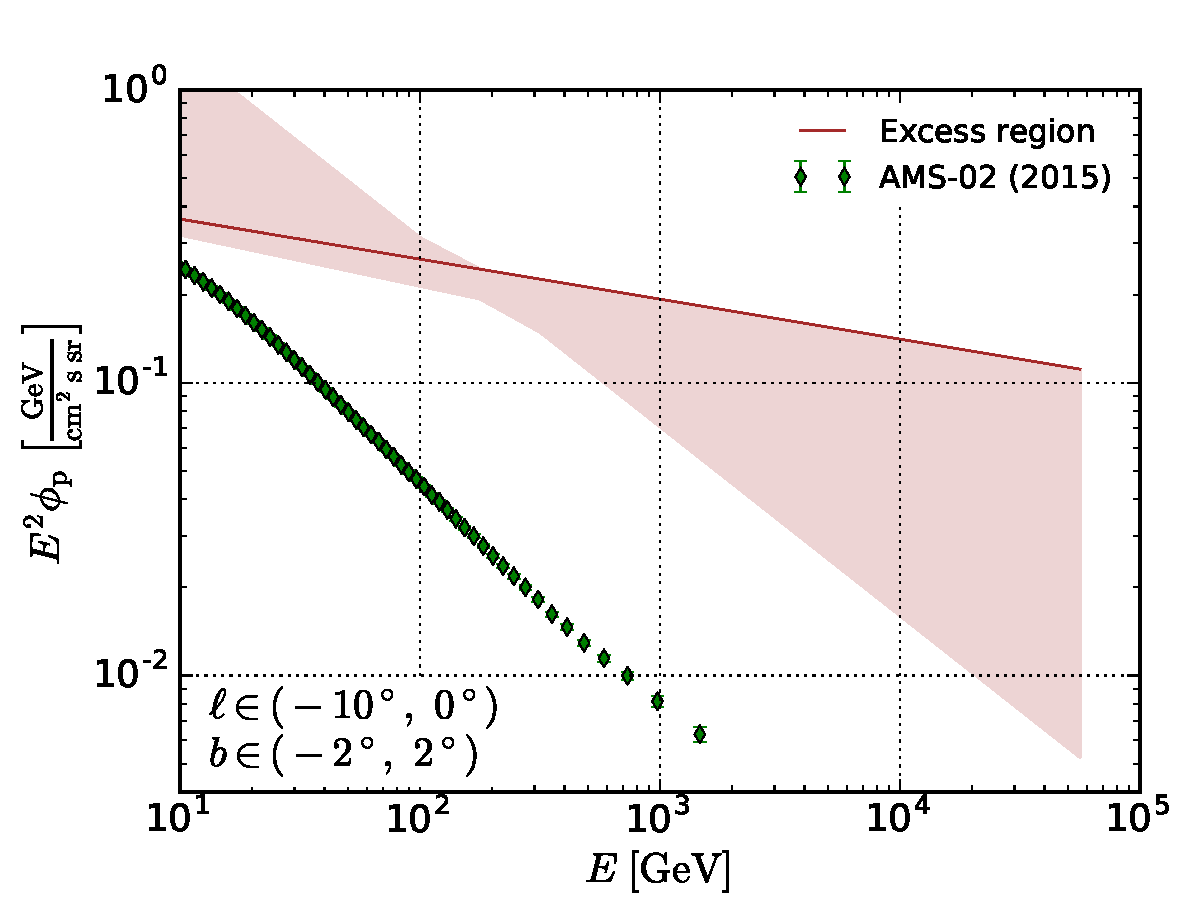
\includegraphics[width=0.5\textwidth]{plots/Summary_proton_spectra_0.pdf}
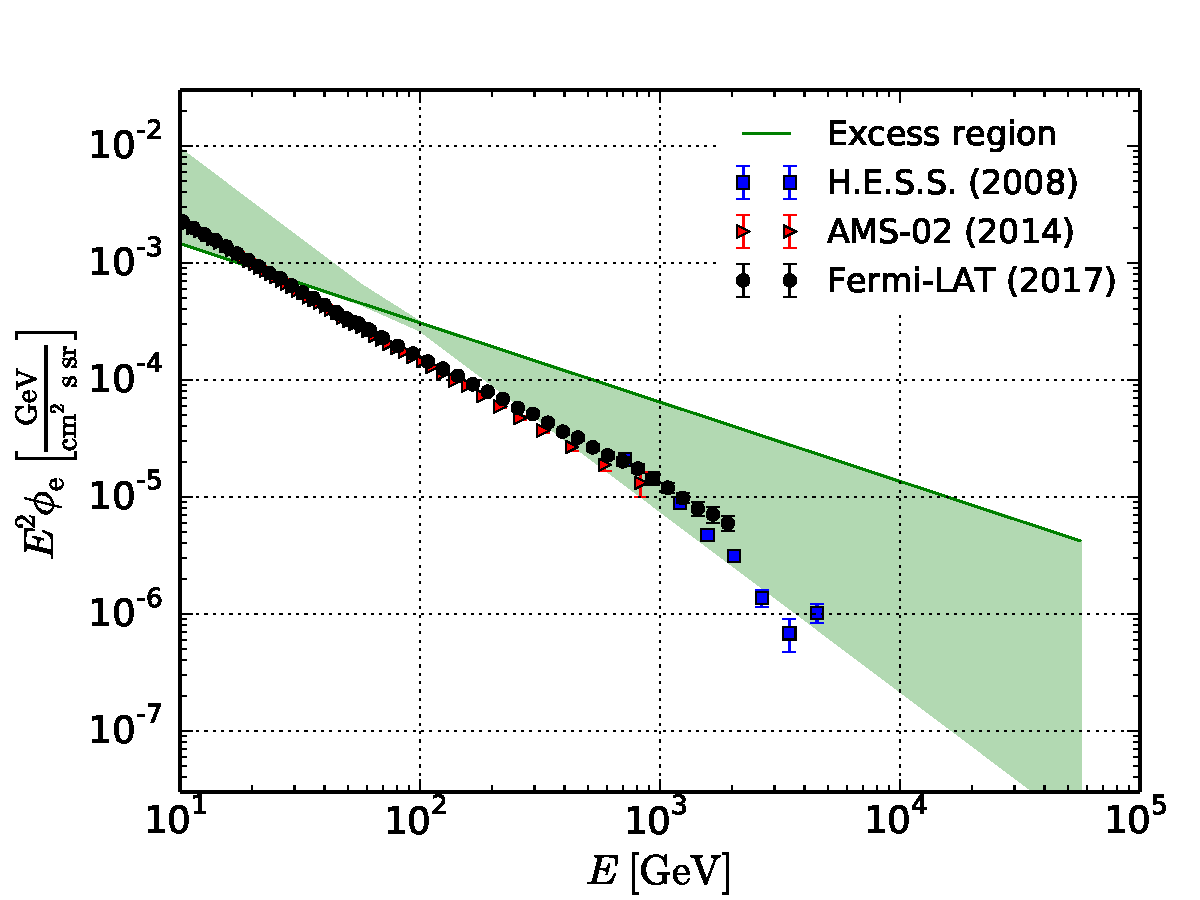
\includegraphics[width=0.5\textwidth]{plots/Summary_electron_spectra_0.pdf}
  	\caption{
	Best-fit proton (left) and electron (right) spectra for the residual plus FBs gamma-ray emission at the base of the FBs.
	Solid lines show the best-fit spectra in the rectangles model of the FBs.
	The shaded bands represent the systematic uncertainties, 
	estimated by the maximal and minimal best-fit FBs spectra among the foreground models. 
	For comparison with the local CR spectrum, data points of some experiments measuring the local CR flux are shown. 
	Here, the error bars represent the combined systematic and statistical uncertainties.}
  	\label{fig:Particle_spectra}
\end{figure*}

\begin{figure}[h]
\centering
 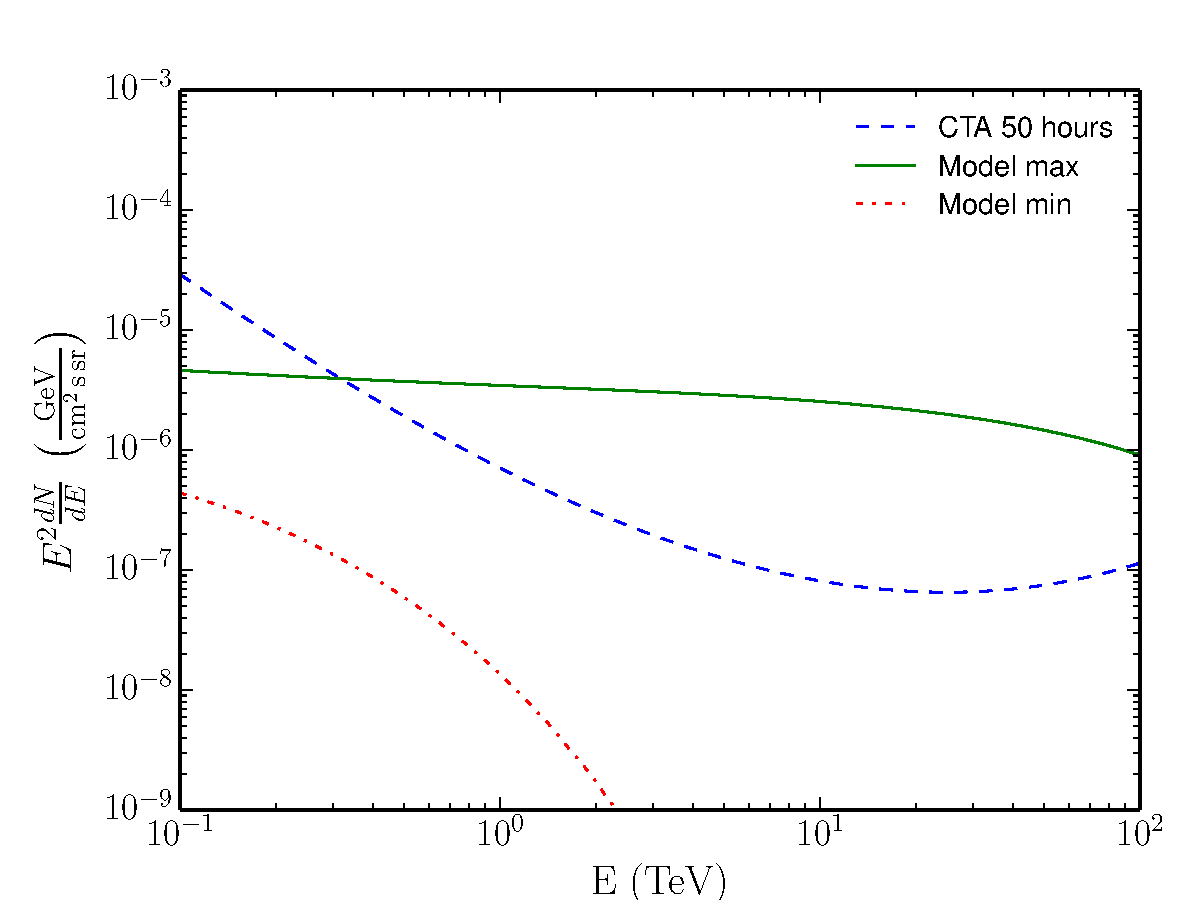
\includegraphics[width=0.48\textwidth]{plots/low_lat_FB_CTA.pdf}
 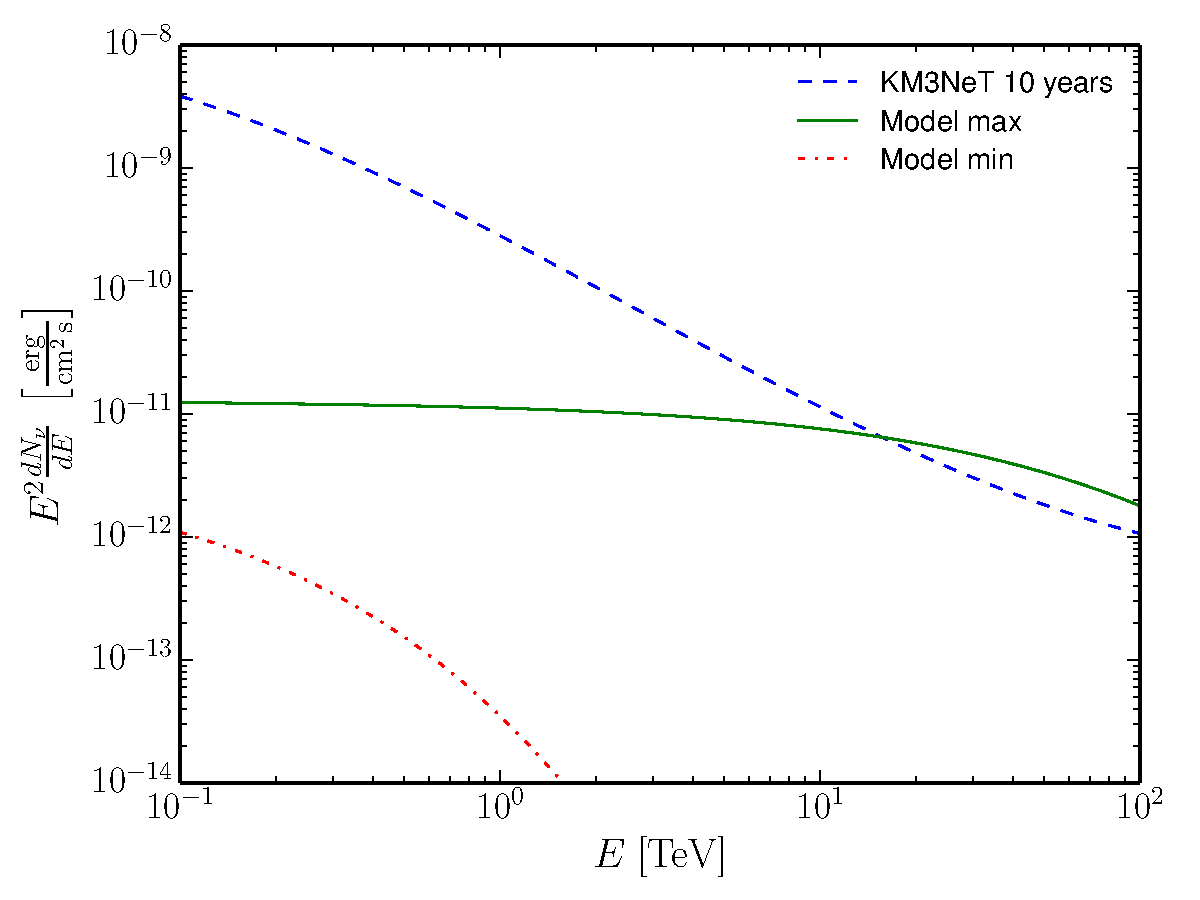
\includegraphics[width=0.48\textwidth]{plots/low_lat_FB_KM3.pdf}
 \caption{Comparison of the hadronic model of the gamma-ray emission at the base of the FBs
 with the sensitivities of CTA and KM3NeT for a source with $2^\circ$ radius \citep{2018APh...100...69A}.
 %For the flux sensitivities we take the estimates of  for a $2^\circ$ radius source and divide by the area of the $2^\circ$ circle to transform to intensity units. 
 The min and max models correspond to the min and max models in
 the hadronic scenario in Table \ref{tab:summary} (for the max model we assume the cutoff in the proton spectrum at 1 PeV)
 integrated over a $2^\circ$ circle to transform intensity to flux.
 The KM3NeT sensitivity is for muon neutrinos only.
 In estimating the sensitivity, we take into account that the GC is below the horizon for about 2/3 of the time
 at the KM3NeT location in the Mediterranean sea.
 }
 \label{fig:sensitivities}
\end{figure}


\subsection{A nearby SNR or a superbubble scenario}

%The position of the hard and bright emission at the base of the FBs can be at any location along the line of sight.
In this subsection we discuss models where the hard and bright gamma-ray emission at the base of the FBs is created either by a single SNR
or several SNRs at a distance closer than the distance to the GC.
We start with a single SNR scenario.
For the leptonic model we use the local ISRF and calculate the IC emission as described in Section \ref{sec:IC_model}.
Assuming one SNR, we find a distance of $\SI{50}{pc}$, which is rather close to Earth and should 
be easily detected in radio and X-ray observations.
For the hadronic model of the gamma-ray emission, we assume that 
the local gas density is similar to the average gas density near the GC \citep{2017ApJ...834...57M}.
At the GC, we need about 700 SNRs, thus the distance where a single SNR can explain the excess emission
is $d = \frac{8.5\: {\rm kpc}}{\sqrt{700}} \approx 300\:{\rm pc}$.
We can compare the flux from the low latitude bubbles with the emission of a known SNR, such as Tycho's SNR.
The SED of Tycho's SNR at 10 GeV is $E^2 {dF}/{dE} \approx 10^{-6}\: {\rm MeV\, cm^{-2} s^{-1}}$ \citep{2017ApJ...836...23A}.
The solid angle of the ROI of $10^\circ \times 12^\circ$ at the base of the FBs is $\Om \approx 0.037$.
If we assume that Tycho's SNR is at a distance of 3 kpc, then the average intensity inside $\Om$ at a distance of 300 pc
is $E^2 {dN}/{dE} \approx 2.7 \times 10^{-6}\: {\rm GeV\, cm^{-2} s^{-1} sr^{-1}}$, which is comparable to the 
FBs emission at latitudes $|b| < 6^\circ$ (e.g., Figure \ref{fig:spec_summary}).
The radius of Tycho's SNR is about 3.5 pc (for the angular diameter of $8'$ at 3 kpc),
while the radius corresponding to $6^\circ$ angular size at 300 pc is about 30 pc, which is almost 10 times larger than the radius of Tycho's SNR.
%It seems unlikely that an SNR can grow to 30 pc radius and keep the population of CR.
If we assume that only the core of the emission at the base of the FBs within $|b| < 2^\circ$ corresponds to an SNR,
the corresponding linear size is $\approx 10$ pc (for the same distance of 300 pc).

Another possibility is that the emission at the base of the FBs is created by several SNRs and / or wind from
massive stars, similar to the Cygnus cocoon \citep{2011Sci...334.1103A} or the local hot bubble.
The Cygnus cocoon \citep{2011Sci...334.1103A} has the radius of about $2^\circ$, 
which at a distance of 1.4 kpc from the Earth, corresponds to a radius of about 50 pc.
If a Cygnus-like region is responsible for the emission within $|b| < 6^\circ$ at the base of the FBs,
then such region should be at a distance of about 500 pc from the Earth.
If only the core of the high intensity region within $|b| < 2^\circ$ is explained by such a cocoon,
then the distance would be similar to the distance to the Cygnus cocoon, i.e., about 1.4 kpc.

\begin{figure}[h]
\centering
 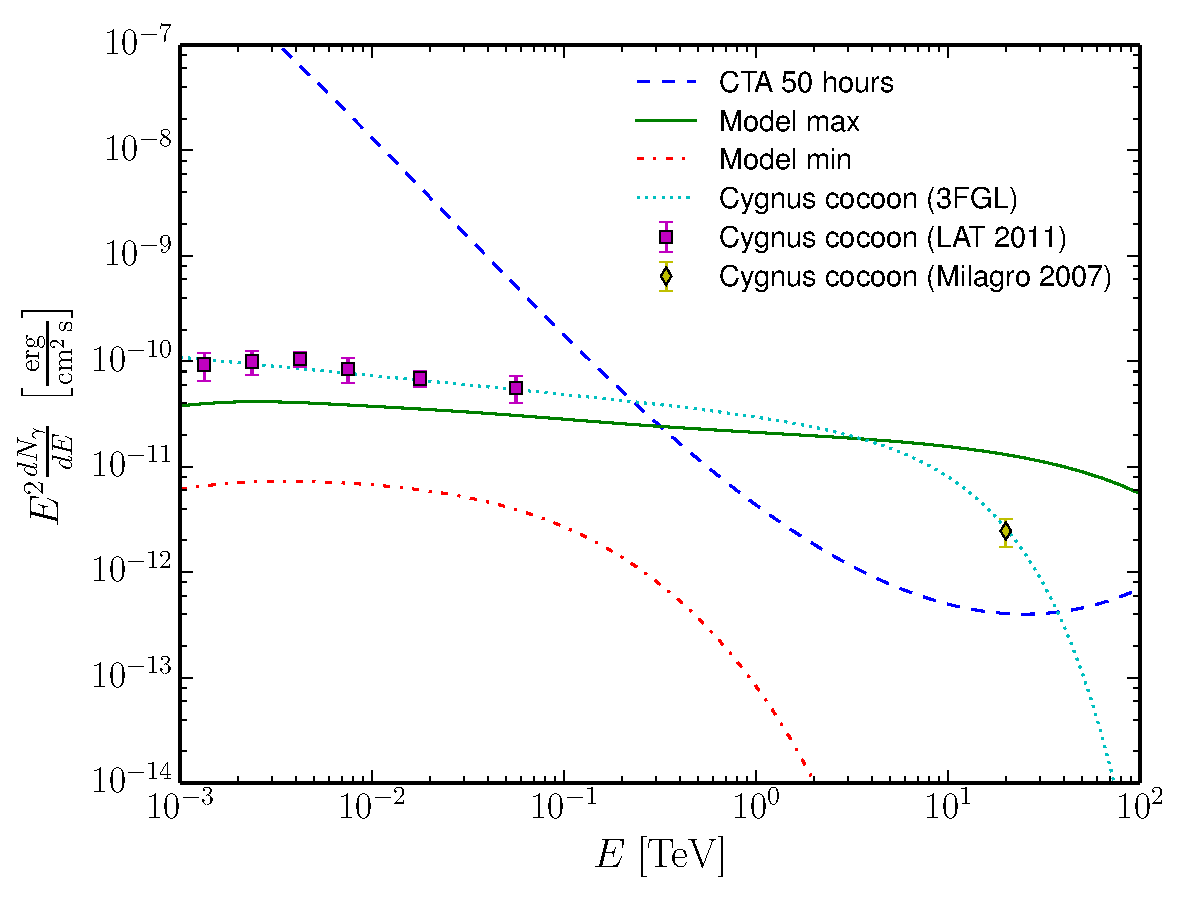
\includegraphics[width=0.48\textwidth]{plots/low_lat_FB_CTA_cygnus.pdf}
 \caption{
 Comparison of the min and max models of the residual flux at the base of the FBs with the Cygnus cocoon spectrum. 
 The min and the max models are the same as in Figure \ref{fig:sensitivities}.
 For the 3FGL spectrum we take the power-law parameters from the catalog \citep{2015ApJS..218...23A}
 and add a cutoff in the gamma-ray spectrum at 10 TeV so that the SED is consistent with the Milagro source MGRO J2031+41 
 at 20 TeV \citep{2007ApJ...664L..91A}.
The purple squares represent the measurement of the flux from the Cygnus cocoon by the \Fermi-LAT collaboration
\citep{2011Sci...334.1103A}.
 }
 \label{fig:cygnus}
\end{figure}


The flux from the Cygnus region around 10 GeV of 
$E^2 {dF}/{dE} \approx 6\times 10^{-5}\: {\rm MeV\, cm^{-2} s^{-1}}$
averaged over a $2^\circ$ circle
corresponds to an intensity of $E^2 {dN}/{dE} \approx 1.6\times 10^{-5}\: {\rm GeV\, cm^{-2} s^{-1}sr^{-1}}$,
which is comparable to the intensity at the base of the FBs within $|b| < 2^\circ$ (Figure \ref{fig:SED_with_fits}),
while the flux from the Cygnus region averaged over a $6^\circ$ circle is comparable to the average intensity
at the base of the FBs within $|b| < 6^\circ$.
Thus the bright gamma-ray emission at the base of the FBs can be explained by a Cygnus-like 
cocoon at a distance of $\sim 500\:{\rm pc} - 1.5 \:{\rm kpc}$ from the Earth towards the GC.
In Figure \ref{fig:cygnus} we compare the SED in the min and max models at $|b| < 2^\circ$
integrated over a $2^\circ$ circle with the SED measured from the Cygnus cocoon 
\citep{2007ApJ...664L..91A, 2011Sci...334.1103A}.
The flux in the max model is comparable (i.e., a factor 2 to 3 smaller) 
to the flux from the Cygnus cocoon between 1 and 100 GeV.

There are several young open stellar clusters in the direction of the base of the FBs, i.e., within $-10^\circ < \ell  < 0^\circ$.
For example, clusters Trumpler 27 \citep{1977ApJ...215..106M} or NGC 6383 \citep{1978MNRAS.184..661L}
contain more than 10 massive OB stars, have an age of about 10 Myr, and an estimated distance of 1.2 kpc and 1 kpc, respectively,
in the direction of $\ell \approx 356^\circ$, $b \approx 0^\circ$.
There is also a cluster NGC 6405 \citep{1959ZA.....47...15R}, which has a smaller estimated distance of about 500 pc
but an older age of about 100 Myr.
The turbulence created by winds from the massive stars as well as the past SNRs in these clusters can (re)accelerate cosmic rays and
it would also lead to smaller diffusion length, which would prevent the escape of CR on timescales shorter than a few Myr \citep{2011Sci...334.1103A}.
There are relatively few SNRs detected in gamma rays in that area of the sky.
In particular, there is only one SNR, 3FGL J1741.1-3053, in the 3FGL catalog \citep{2015ApJS..218...23A}
between $-10^\circ < \ell  < 0^\circ$.
This SNR is associated with Tornado nebula at a distance of 12 kpc from Earth \citep{2013ApJ...774...36C}.
Green's catalog of SNRs \citep{2014BASI...42...47G, 2017Green} contains several SNRs between $-10^\circ < \ell  < 0^\circ$,
but SNRs with measured distances are more than 4 kpc away.
The absence of detected SNRs in the direction of the base of the FBs at the distance $\lesssim 1.5$ kpc 
does not necessarily mean that there were no SNRs in the open clusters mentioned above.
The reason is that the wind from the massive stars as well as the first SNRs in the cluster create a hot superbubble
with smaller gas density than the average density in the Galactic plane, as a result the subsequent SNRs quickly expand
in the less dense environment until they reach the common envelope of the superbubble 
\citep[see, e.g., simulations of the formation of the local hot superbubble and the possible scenario of the Loop I formation in][]%
{2016Natur.532...73B, 2017A&A...604A..81S, 2018Galax...6...26S}.
Whether the stellar clusters can provide the necessary CR injection rate to power the gamma-ray emission at the base
of the FBs deserves a separate detailed study.

An interesting question is whether the FBs themselves can be inflated by a Cygnus-like superbubble,
which accidentally happened along the line of sight towards the GC.
If the FBs are at a distance of about 1 kpc, then their vertical size is also about 1 kpc,
which is 10 times smaller than the size of the FBs at a distance of 8.5 kpc.
In the leptonic scenario of the FBs, the $10^{52}$ erg in CRe at 8.5 kpc \citep{2014ApJ...793...64A}
would correspond to $10^{50}$ erg at 1 kpc.
This power can be provided by several hundred SNe, which is a relatively large number, given the few young stellar 
clusters at distances $\lesssim$ 1 kpc from Earth in the direction of the base of the FBs.
This estimate assumes the 0.1\% efficiency in acceleration of CRe by SN shells,
if there is an additional acceleration of the electrons by the turbulence either at the base of the FBs
or inside the high latitude FB volume, then the required number of SNRs would be smaller.

The electrons can be delivered to the FBs volume by an outflow,
possibly, created by the pressure of the CR themselves \citep[e.g.,][]{2018MNRAS.475..570J}.
The measured outflow velocities in the direction of the FBs are on the order of 1000 km/s
with an age of the outflow at the position above the GC about 6 - 9 Myr \citep{2015ApJ...799L...7F, 2017ApJ...834..191B}.
If the distance is 10 times smaller, then the age would be $\sim 600 - 900$ kyr,
which is comparable to the cooling time of 1 TeV electrons necessary to explain the 
gamma-ray emission from the FBs at high latitudes \citep{2014ApJ...793...64A}.
Thus the gamma-ray emission at high latitudes can be explained by IC model with about 100 SNRs
created $\sim$ 1 Myr ago, while the bright and hard emission at the base of the bubbles can
be explained by the hadronic emission from about 10 SNRs. 
The actual age of the system is determined by the confinement within the superbubble and can be also on the order
of 1 Myr or more.
In this scenario,
the star forming region, which can power the emission at the base of the FBs and, possibly, the FBs themselves
can be situated in the Sagittarius arm at a distance of 1 -- 1.5 kpc in the direction of the GC.


\section{Conclusions}

In the paper we use 9 years of \Fermi-LAT Source class data to study the gamma-ray emission
at the base of the FBs.
We use different methods to construct the foreground diffuse gamma-ray emission and to determine
the properties of the residual gamma-ray emission.
We confirm the earlier findings that the emission at the base of the FB
has a higher intensity than the FBs emission at high latitudes.
The spectrum is consistent with a single power law without a cutoff up to about 1 TeV.
The emission is slightly displaced from the GC to negative longitudes,
which favors a starburst scenario of the bubbles formation, unless there is a mechanism to shift the
gamma-ray emission away from Sgr A* in the SMBH scenario.

The gamma-ray emission at the base of the FBs can be explained by either a hadronic or a leptonic model of gamma-ray production
with CR spectra consistent with a power law without a cutoff.
The index of the CRe (CRp) spectrum is 2.6 -- 2.7 (2.0 -- 2.1).
We derive the 95\% confidence lower bound on the cutoff in the CR electron and proton spectra
by selecting the lowest 95\% statistical confidence among the different models of the foreground emission.
Within $|b| < 2^\circ$ and $-10^\circ < \ell < 0^\circ$, the 95\% confidence lower bound on the CRe (CRp) spectrum is
about 3 (6) TeV.
If we instead fit the leptonic and hadronic models to the lowest points in the modeling uncertainty
envelope (although these points may
come from different foreground models), then the minimal cutoff in the leptonic (hadronic) model
is estimated as 0.4 (1.1) TeV.

If the location of the residual emission is near the GC,
then the total gamma-ray luminosity is $L \approx 10^{37}\ {\rm erg\ s^{-1}}$,
the required energy of CRe (CRp) above 1 GeV is $E_{\rm e} = \SI{3e51}{erg}$
($E_{\rm p} = \SI{7e52}{erg}$).
Although the total required energy in CRe is smaller than in CRp,
the efficiency of acceleration of hadronic CR is expected to be significantly higher than for leptonic CR.
In particular, with 10\% CRp acceleration efficiency, one needs about 700 SNRs to explain the 
gamma-ray emission in the hadronic scenario near the GC,
while with 0.1\% CRe acceleration efficiency, the required number of SNRs is 3000.
If the residual gamma-ray emission is produced at a closer distance, e.g., at about 1 kpc
by a Cygnus-like cocoon or a superbubble in the Sagittarius arm, 
then the required number of SNRs is about two orders of magnitude smaller.

For the GC scenario, the diffusive escape time and the electron cooling time is $\sim 200$ kyr.
In this case one needs a relatively high SN rate of one per $\sim$ 200 yr at the location of the gamma-ray emission.
For the superbubble scenario, the characteristic linear size is 10 times smaller, which leads to 100 times shorter
diffusion time of a few kyr. This is shorter than the lifetime of individual SNRs.
In this case, the age of the CR population can be longer than the diffusion time if there is an
additional confinement by the SN shells or the shell of the superbubble.
Together with the question of the location of the residual emission at the base of the FBs,
one can revisit the question of the location of the FBs themselves:
the FBs could have been inflated by a superbubble about 1 Myr ago
at a distance of 1 kpc from the Sun.
The CR in the past superbubble may create a wind with velocities up to $\sim$ 1000 km/s, 
which are sufficient to inflate a 1 kpc large bubble within 1 Myr
so that the CR electrons in the wind do not cool below 1 TeV and can explain the
gamma-ray emission from the FBs at high latitudes.
The gamma-ray emission at low latitudes is then explained (most naturally) by a hadronic
scenario from a different and more recent starburst episode at about the same location.

In the future, the bright and hard gamma-ray emission at the base of the FB
should be detectable with the CTA telescopes, or a version of the HAWC experiment in the southern hemisphere 
\citep{2017APS..APR.R4005M, 2017arXiv170909624A}.
Observations with Cherenkov telescopes should detect or put constraints on the cutoff value in the gamma-ray spectrum in multi-TeV regime.
In the hadronic scenario, for a sufficiently high cutoff value of the CRp spectrum, e.g., around 1 PeV,
the corresponding neutrino emission can be detected with the future KM3NeT telescope.


\subsection*{Acknowledgements}

The authors would like to thank Anna Franckowiak, Stefan Funk, Tsunefumi Mizuno, Andrew Strong, and Luigi Tibaldo for valuable comments and suggestions.
The Fermi LAT Collaboration acknowledges generous ongoing support from a number of agencies and institutes that have supported both the development and the operation of the LAT as well as scientific data analysis. These include the National Aeronautics and Space Administration and the Department of Energy in the United States, the Commissariat à l'Energie Atomique and the Centre National de la Recherche Scientifique / Institut National de Physique Nucléaire et de Physique des Particules in France, the Agenzia Spaziale Italiana and the Istituto Nazionale di Fisica Nucleare in Italy, the Ministry of Education, Culture, Sports, Science and Technology (MEXT), High Energy Accelerator Research Organization (KEK) and Japan Aerospace Exploration Agency (JAXA) in Japan, and the K. A. Wallenberg Foundation, the Swedish Research Council and the Swedish National Space Board in Sweden.




